\chapter{Implementierung}


Die Implementierung des Projekts lässt sich in vier Bereiche unterteilen: Die Baumrepräsentation enthält Daten, die von den L-System und Space Colonization Implementierungen generiert werden. Diese Daten werden an das Modellgenerierungssystem übergeben, welches die Modelldaten für eine grafische Darstellung in der Unreal Engine 4 produziert.


\section{Baumrepräsentation}

Der Space Colonization Algorithmus generiert einen Baum-Graphen, auf Grundlage dessen die Modellgenerierung durchgeführt wird. Auch die Aktionen, welche von einer Turtle ausgeführt werden, können, wie in Abschnitt \ref{subsec:TurtleInterpretationImplementation} beschrieben, in einem Baum-Graphen gespeichert werden. Die implementierte Baumrepräsentation kann daher von beiden Systemen verwendet werden und ermöglicht es, diese mit demselben Modellgenerierungssystem zu visualisieren.

Die Baumstruktur wird durch eine Datenklasse repräsentiert, jedes Objekt dieser Klasse beschreibt einen Knoten sowie die Kante, welche vom Vorgänger zu dem Knoten führt. Die Datenklasse bietet Zugriff auf die folgenden Informationen:

\begin{description}
	\item \textbf{Vorgänger und Nachfolger:} Mithilfe eines Verweises auf den Vorgänger und eine Liste der Nachfolger eines Knotens kann der Baum-Graph vollständig repräsentiert werden. Weiterhin ermöglicht dies die Implementierung einer Reihe von rekursiven Funktionen zur Anpassung von Modelldaten.\\
	
	\item \textbf{Modell-Daten:} Kanten werden, wie in Abschnitt \ref{subsec:ZylinderMeshes} beschrieben, mithilfe von Zylindern visualisiert. Um die Generierung von Modelldaten zu vereinfachen, bietet die Datenklasse Zugriff auf Start- und Endposition, Start- und Endradius, Start- und Endnormale sowie einen Rotationswinkel. 
	
	Weiterhin wird die Zweigtiefe des repräsentierten Knoten gespeichert.\\
	
	\item \textbf{Wachstums-Daten:} Die Wachstums-Daten bestehen aus einer Wachstumsrichtung, einem Einfluss-Zähler und dem \glqq Kein Wachstum\grqq-Zähler ($NG$-Counter), welche für den Ablauf des Space Colonization Algorithmus benötigt werden.	
\end{description}

\section{L-Systeme}

Die Implementierung von L-Systemen wird durch einen Unreal-Akteur verwirklicht, der im Level platziert werden kann. Nach Start des Levels wird das angegebene Axiom anhand der Produktionsregeln abgeleitet und die sich ergebende Zeichenkette von der Turtle-Implementierung interpretiert.

\subsection{Parameter}

Dem L-System-Akteur werden die folgenden Parameter über die Editor-UI übergeben:

\begin{description}
	\item \textbf{Anzahl der Ableitungen:} Die Anzahl der Ableitungen in $\mathbb{N}^+$, die auf dem Axiom durchgeführt werden sollen. \\
	
	\item \textbf{Axiom:} Das Axiom in Form einer Zeichenkette. \\
	
	\item \textbf{Konstanten:} Eine Konstante besteht aus der Angabe eines Identifikationssymbols und eines Wertes in $\mathbb{R}$. Konstanten können im Axiom und in den Nachfolgern der Produktionen verwendet werden.\\	
	
	\item \textbf{Produktionen:} Jede Produktion besteht aus Angabe eines Vorgängers, eine Liste von Parametern und einem Nachfolger. Der Vorgänger und jeder Parameter entspricht einem einzelnen Symbol, der Nachfolger wird als Zeichenkette eingetragen. Die Parametersymbole können nur innerhalb des Nachfolgers verwendet werden. Der Vorgänger und die Liste der Parameter bilden das parametrische Wort, welches bei einer Ableitung durch den Nachfolger ersetzt wird.
\end{description}
\begin{figure} [hbtp]
	\centering
	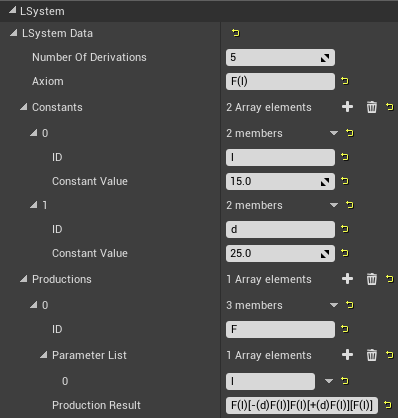
\includegraphics[height=0.4\textheight]{images/LS_ExampleUE4UI.png}
	\caption{Ein Beispiel für die Angabe des L-Systems aus Gleichung \ref{eq:ProdBranching2} mit der resultierenden Baumstruktur aus Abbildung \ref{fig:Branching2L15D25}.}
	\label{fig:LS_ExampleUE4UI}
\end{figure}
Für das Axiom und die Produktionen gelten die in Kapitel \ref{ch:LSysteme} festgelegten Regeln für die Definition von L-Systemen. Weiterhin gelten die üblichen Regeln für die Angabe von arithmetischen Operationen. Die Verwendung von Klammern ist jedoch auf die Angabe von Parametern eines parametrischen Wortes beschränkt, ihre Verwendung zur Beeinflussung der Auswertungsreihenfolge eines arithmetischen Ausdrucks wird nicht unterstützt.

Ein Beispiel für die korrekte Eingabe eines L-Systems über die Editor-UI wird in Abbildung \ref{fig:LS_ExampleUE4UI} gezeigt.

\subsection{Ableitung}

Zu Anfang der Erstellung des L-System-Akteurs werden alle Konstantensymbole im Axiom und den Produktionen durch die Konstantenwerte ersetzt. 

Die Implementierung arbeitet durchgehend auf derselben Zeichenkette, angefangen mit dem Axiom. In jeder Ableitung werden die in den Produktionsregeln definierten parametrischen Wörter durch die angegebenen Nachfolger ersetzt.

Nachdem die vorgegebene Anzahl von Ableitungen durchgeführt wurde, wird die resultierende Zeichenkette an die Turtle-Implementierung weiter gegeben.

\subsection{Turtle Interpretation} \label{subsec:TurtleInterpretationImplementation}



Was passiert hier?

Erweiterung der Turtle Interpretation, um 



Die Aktionen der Turtle für die Modellgenerierung als Baum gespeichert werden. \cite[S.21]{ABOP:04} 

\section{Space-Colonization Algorithmus}

\subsection{Parameterübergabe}

\subsection{Einflussbereich}

\subsection{Ablauf des Algorithmus}


\section{Modellgenerierung} \label{sec:Modellgenerierung}

\subsection{Parameterübergabe}

\subsection{Procedural Mesh Component}

\subsection{Generierung der Zylinder-Meshes} \label{subsec:ZylinderMeshes}

Die Startposition entspricht der Endposition des Vorgängers und markiert den Anfang der Kante, die zu dem Knoten führt, der durch das Datenobjekt beschrieben wird. Die Endposition beschreibt die Position des Knotens und markiert das Ende der Kante, die zu dem Knoten führt. 

Der Startradius bestimmt den Radius des Start-Zylinderrings, Startposition und Startnormale beschreiben die Ebene, auf welcher der Zylinderring generiert wird. Der Endradius entspricht dem Radius des End-Zylinderrings, Endposition und Startnormale beschreiben die Ebene, auf welcher der Ring erstellt wird.

\subsection{Operationen auf der Baumstruktur}

Was kann mit BranchUtility gemacht werden?
